%==============================================================================
% PAPER 6, CHAPTER 2: Zero-Point Energy Extraction
%==============================================================================

\chapter{Zero-Point Energy Extraction}
\label{ch:p6:zpe_extraction}

%------------------------------------------------------------------------------
\section{Introduction: The Casimir Promise}
%------------------------------------------------------------------------------

\openingquote{%
``The energy of the electromagnetic field in a volume bounded by perfectly conducting walls differs from that of the same field in free space.''%
}{Hendrik Casimir, 1948}

\marginnote{historical-context}{%
Casimir predicted vacuum fluctuations create attractive force between neutral conducting plates, experimentally confirmed in 1997 by Lamoreaux to 5\% accuracy.%
}

In 1948, Hendrik Casimir derived a startling result: two uncharged parallel conducting plates separated by distance $d$ experience attractive force proportional to $d^{-4}$, arising purely from quantum vacuum fluctuations\cite{Casimir1948}. The Casimir effect demonstrated that zero-point energy (ZPE)---lowest possible energy state of quantum fields---has measurable physical consequences.\marginnote{physical-intuition}{%
Conducting boundaries alter vacuum mode density: fewer allowed wavelengths between plates than outside, creating pressure imbalance.%
}

The standard Casimir force per unit area between ideal conductors:\marginnote{theoretical-prediction}{%
Force becomes significant at nanometer separations: $F/A \sim 1$ atm for $d \sim 10$ nm, dominating van der Waals attraction.%
}

\begin{equation}
  \frac{F}{A} = -\frac{\hbar c \pi^2}{240 d^4}
  \label{eq:p6:casimir_force}
\end{equation}

The negative sign indicates attraction. At separation $d = 1~\mu$m: $F/A \approx -13$ mPa; at $d = 10$ nm: $F/A \approx -1.3 \times 10^5$ Pa $\approx 1$ atmosphere. This is a \textit{conservative} force derivable from potential energy $U(d) \propto -d^{-3}$, implying extracting energy requires external work to separate plates.\marginnote{energy-conservation}{%
Moving plates apart stores energy in ZPE field configuration; no violation of conservation laws despite ``vacuum energy extraction'' language.%
}

\textbf{The extraction challenge:} Can non-conservative Casimir-like configurations produce \textit{directional} thrust or sustained power output? Three proposed mechanisms:\marginnote{research-frontiers}{%
Dynamic Casimir effect (DCE) confirmed experimentally by Wilson et al. (2011) in superconducting circuits, validating photon creation from vacuum modulation.%
}

\begin{enumerate}
  \item \textbf{Dynamic Casimir Effect (DCE):} Time-varying boundaries convert virtual photons to real photons, extracting ZPE at cost of mechanical work.

  \item \textbf{Metamaterial Resonators:} Engineered electromagnetic environments with negative refractive index modify vacuum mode density, enabling directional energy flow.

  \item \textbf{Parametric Amplification:} Modulating circuit parameters (capacitance, inductance) at resonance frequencies amplifies vacuum fluctuations into detectable signals.
\end{enumerate}

This chapter quantifies these mechanisms, evaluates theoretical limits (Bekenstein bound, Landauer principle), calculates realistic power outputs, and assesses technological feasibility. \textit{Caveat}: All proposed ZPE extraction schemes face severe thermodynamic and practical constraints; we provide honest assessments.

%------------------------------------------------------------------------------
\section{Theoretical Limits and Conservation Laws}
%------------------------------------------------------------------------------

\subsection{Bekenstein Bound on Extractable Energy}

The Bekenstein bound relates maximum information (hence energy) in a finite region to its surface area\cite{Bekenstein1981}:\marginnote{information-theoretic-limit}{%
Bound prevents infinite information density, underpinning holographic principle and black hole thermodynamics.%
}

\begin{equation}
  I \leq \frac{2\pi R E}{\hbar c \ln 2}
  \label{eq:p6:bekenstein_bound}
\end{equation}

where $I$ is information content (bits), $R$ is radius of sphere enclosing system, $E$ is total energy (including rest mass). For electromagnetic ZPE in volume $V = \frac{4}{3}\pi R^3$:\marginnote{application-to-zpe}{%
ZPE density formally diverges due to infinite frequency modes; regularization via Bekenstein bound provides physical cutoff.%
}

\begin{equation}
  E_{\text{ZPE}} \leq \frac{\hbar c \ln 2}{2\pi} \cdot \frac{I}{R}
  \label{eq:p6:zpe_bekenstein}
\end{equation}

\textbf{Example:} For $R = 1$ m sphere and $I = 10^{80}$ bits (observable universe information content), maximum ZPE:\marginnote{numerical-estimate}{%
Using $\hbar c = 1.97 \times 10^{-25}$ J·m: $E_{\text{max}} \sim 10^{55}$ J, vastly exceeding total matter-energy in observable universe ($\sim 10^{70}$ J). Bound is weak for macroscopic volumes.%
}

\begin{equation}
  E_{\text{max}} \sim \frac{10^{-34} \times 3 \times 10^8 \times 0.693}{6.28} \times \frac{10^{80}}{1} \sim 10^{54} \text{ J}
  \label{eq:p6:bekenstein_example}
\end{equation}

The Bekenstein bound does not prohibit ZPE extraction but requires extracted energy be compensated by increased entropy elsewhere (Second Law compliance).\marginnote{thermodynamic-constraint}{%
Extracting ordered energy from vacuum fluctuations necessitates entropy increase in environment (heat dissipation), limiting efficiency.%
}

\subsection{Landauer Principle and Irreversible Computation}

Landauer's principle states: erasing one bit of information requires minimum energy dissipation:\marginnote{information-erasure}{%
Principle sets fundamental limit on energy efficiency of computation, independent of implementation technology.%
}

\begin{equation}
  E_{\text{erase}} \geq k_B T \ln 2
  \label{eq:p6:landauer_principle}
\end{equation}

where $k_B$ is Boltzmann constant, $T$ is temperature. At room temperature ($T = 300$ K): $E_{\text{erase}} \geq 2.9 \times 10^{-21}$ J/bit.\marginnote{room-temp-limit}{%
Modern CMOS transistors dissipate $\sim 10^{-15}$ J per operation, six orders of magnitude above Landauer limit due to irreversible logic gates.%
}

\textbf{Connection to ZPE extraction:} Harnessing vacuum fluctuations requires \textit{measurement} of fluctuation states (determining whether virtual photon is present), followed by \textit{amplification} (converting virtual to real). Measurement collapses quantum state, erasing information about original superposition. Total energy cost:\marginnote{measurement-backaction}{%
Quantum measurement disturbs system; energy extracted from vacuum must exceed measurement back-action to achieve net gain.%
}

\begin{equation}
  E_{\text{cost}} = N_{\text{bits}} k_B T \ln 2 + E_{\text{measurement}}
  \label{eq:p6:extraction_cost}
\end{equation}

where $N_{\text{bits}}$ is information gathered, $E_{\text{measurement}}$ is quantum measurement back-action energy. For $N_{\text{bits}} \sim 10^{10}$ (monitoring $\sim$GHz modes for 1 s), $E_{\text{cost}} \sim 10^{-11}$ J at 300 K.\marginnote{efficiency-estimate}{%
Extracted ZPE energy must exceed $10^{-11}$ J to break even; realistic devices extract $\sim 10^{-15}$ J per cycle (insufficient).%
}

%------------------------------------------------------------------------------
\section{Dynamic Casimir Effect: Photon Generation from Motion}
%------------------------------------------------------------------------------

\subsection{Moving Mirror Model}

The dynamic Casimir effect (DCE) describes photon pair creation from vacuum when cavity boundary moves at relativistic speeds\cite{Moore1970}. For mirror oscillating at position $d(t) = d_0 + d_1 \cos(\omega_m t)$:\marginnote{time-varying-boundary}{%
Oscillating boundary modulates cavity resonance frequency, parametrically amplifying vacuum fluctuations into real photons.%
}

\begin{equation}
  d(t) = d_0 \left(1 + \beta \cos(\omega_m t)\right), \quad \beta = d_1 / d_0 \ll 1
  \label{eq:p6:oscillating_mirror}
\end{equation}

Cavity resonance frequency: $\omega_n = n\pi c / d(t)$ becomes time-dependent. Photon creation rate for mode $n$:\marginnote{photon-emission}{%
Photons created in pairs with total energy $2\hbar \omega_n$, conserving momentum via mirror recoil.%
}

\begin{equation}
  \frac{dN_n}{dt} = \frac{\beta^2 \omega_m^3}{c^3} \left(\frac{c}{d_0}\right)^3 \delta(\omega_m - 2\omega_n)
  \label{eq:p6:dce_photon_rate}
\end{equation}

The delta function enforces resonance condition: mirror frequency $\omega_m$ must match twice the cavity mode frequency $2\omega_n$ (photon pairs have equal frequency $\omega_n$).\marginnote{resonance-condition}{%
Off-resonance photon creation exponentially suppressed; requires precise frequency matching to within $\sim 0.1\%$.%
}

\textbf{Power extraction:} Each photon pair carries energy $2\hbar \omega_n$. Total power:\marginnote{power-scaling}{%
Power scales as $\beta^2 \omega_m^3$: cubic dependence on modulation frequency demands GHz-THz operation.%
}

\begin{equation}
  P_{\text{DCE}} = \sum_n \frac{dN_n}{dt} \times 2\hbar \omega_n \approx \frac{\beta^2 \omega_m^4 d_0^3}{c^3} \hbar
  \label{eq:p6:dce_power}
\end{equation}

\textbf{Numerical example:} For $d_0 = 1~\mu$m, $\beta = 0.1$, $\omega_m = 2\pi \times 10$ GHz:\marginnote{realistic-parameters}{%
Amplitude $d_1 = 0.1~\mu$m, velocity $v_{\text{max}} = \omega_m d_1 \sim 6$ m/s (non-relativistic), yet photon creation remains quantum effect.%
}

\begin{align}
  P_{\text{DCE}} &\approx \frac{(0.1)^2 (6 \times 10^{10})^4 (10^{-6})^3}{(3 \times 10^8)^3} \times 10^{-34} \nonumber\\
  &\approx 10^{-18} \text{ W}
  \label{eq:p6:dce_power_example}
\end{align}

Minuscule power output. Mechanical work to oscillate mirror:\marginnote{energy-balance}{%
Damping force from photon emission back-reacts on mirror, requiring continuous energy input to maintain oscillation.%
}

\begin{equation}
  P_{\text{mechanical}} = F_{\text{damping}} \times v_{\text{max}} \sim \frac{P_{\text{DCE}}}{c} \times c = P_{\text{DCE}}
  \label{eq:p6:mechanical_power}
\end{equation}

Net energy extraction: zero (energy merely transduced from mechanical to electromagnetic form, no ``free'' ZPE harvesting).

\subsection{Experimental Realization: Superconducting Circuits}

Wilson et al. (2011) demonstrated DCE in superconducting circuit where effective cavity length modulated via SQUID (superconducting quantum interference device) tuned by magnetic flux\cite{Wilson2011}.\marginnote{experimental-breakthrough}{%
First direct observation of DCE photon creation, confirming 60-year-old theoretical prediction.%
}

\textbf{Setup:} Coplanar waveguide resonator terminated by SQUID, effective inductance $L(\Phi) = L_0 / \cos(\pi \Phi / \Phi_0)$ where $\Phi$ is applied flux, $\Phi_0 = h/(2e)$ is flux quantum. Modulating $\Phi(t)$ changes resonance frequency:\marginnote{tunable-resonator}{%
SQUID acts as tunable inductor, varying effective cavity length without mechanical motion.%
}

\begin{equation}
  \omega_{\text{res}}(t) = \frac{1}{\sqrt{L(\Phi(t)) C}} = \omega_0 \left[1 + \frac{\beta}{2}\cos(\omega_m t) + O(\beta^2)\right]
  \label{eq:p6:squid_resonance}
\end{equation}

where $\beta \sim 0.05$ (5\% modulation depth). Operating at $\omega_0 / 2\pi \sim 10$ GHz, measured photon creation rate:\marginnote{measured-output}{%
Detected $\sim 0.5$ photons per modulation cycle at optimal flux modulation, confirming DCE photon creation.%
}

\begin{equation}
  \frac{dN}{dt} \sim 0.5 \times 10^{10} \text{ photons/s}
  \label{eq:p6:wilson_photon_rate}
\end{equation}

Power output: $P = (dN/dt) \times \hbar \omega_0 \sim 0.5 \times 10^{10} \times 10^{-34} \times 6 \times 10^{10} \sim 3 \times 10^{-13}$ W.\marginnote{sub-picowatt}{%
300 femtowatts---detectable by cryogenic amplifiers but insufficient for macroscopic energy harvesting.%
}

Input power (flux modulation drive): $P_{\text{in}} \sim 10^{-10}$ W (estimated from flux bias circuit dissipation). Efficiency: $\eta \sim 0.3\%$ (most input power dissipated as heat, not converted to photons).\marginnote{thermodynamic-loss}{%
Resistive losses in flux control circuitry overwhelm DCE photon energy output by $\sim$300:1 ratio.%
}

%------------------------------------------------------------------------------
\section{Metamaterial Resonators}
%------------------------------------------------------------------------------

\subsection{Negative Index Materials and Vacuum Engineering}

Metamaterials---artificially structured composites with electromagnetic properties not found in nature---enable engineering of vacuum mode density\cite{Pendry2006}. Key property: \textit{negative refractive index} $n < 0$, requiring simultaneous negative permittivity $\epsilon < 0$ and permeability $\mu < 0$.\marginnote{double-negative-condition}{%
Standard materials: $n = +\sqrt{\epsilon \mu}$. Metamaterials: $n = -\sqrt{\epsilon \mu}$ (negative root selected by causality).%
}

\textbf{Dispersion relation in metamaterial:}\marginnote{backward-wave-propagation}{%
Phase velocity $\mathbf{v}_p$ antiparallel to group velocity $\mathbf{v}_g$, creating ``left-handed'' electromagnetic waves.%
}

\begin{equation}
  \mathbf{k} = -\frac{\omega}{c} n(\omega) \hat{\mathbf{n}}
  \label{eq:p6:metamaterial_dispersion}
\end{equation}

where $\hat{\mathbf{n}}$ is propagation direction. Negative $n$ reverses wavevector direction relative to energy flow (Poynting vector).\marginnote{energy-flow}{%
Energy flows forward ($\mathbf{S} = \mathbf{E} \times \mathbf{H}$) while phase fronts move backward ($\mathbf{k}$ antiparallel).%
}

\subsection{Casimir Force Modification in Metamaterial Cavities}

Leonhardt \& Philbin (2007) showed metamaterial boundaries can invert Casimir force from attractive to \textit{repulsive}\cite{Leonhardt2007}. For plates with permittivity $\epsilon_1, \epsilon_2$ in vacuum:\marginnote{repulsive-casimir}{%
Repulsive Casimir force between dissimilar materials enables vacuum pressure-driven actuators without external power.%
}

\begin{equation}
  \frac{F}{A} = -\frac{\hbar c \pi^2}{240 d^4} \times \mathcal{F}(\epsilon_1, \epsilon_2)
  \label{eq:p6:metamaterial_casimir}
\end{equation}

where $\mathcal{F}(\epsilon_1, \epsilon_2)$ is material-dependent factor. For $\epsilon_1 > 0, \epsilon_2 < 0$ (one normal, one metamaterial): $\mathcal{F} < 0$, reversing sign of force.\marginnote{sign-reversal}{%
Physical origin: metamaterial supports different vacuum mode spectrum than ordinary material, inverting radiation pressure balance.%
}

\textbf{Thrust generation:} Asymmetric cavity with one metamaterial plate and one normal conductor experiences net force:\marginnote{directional-thrust}{%
Repulsive side pushes harder than attractive side pulls, creating imbalance exploitable for propulsion.%
}

\begin{equation}
  F_{\text{net}} = F_{\text{repulsive}} - F_{\text{attractive}} \sim \frac{\hbar c \pi^2}{240} \left(\frac{1}{d_1^4} - \frac{1}{d_2^4}\right)
  \label{eq:p6:asymmetric_thrust}
\end{equation}

For $d_1 = 10$ nm (repulsive gap), $d_2 = 100$ nm (attractive gap): $F_{\text{net}} \sim 10^{-8}$ N per cm$^2$ of plate area.\marginnote{thrust-magnitude}{%
At 1 m$^2$ total area: $F \sim 10^{-4}$ N---6 orders of magnitude below chemical rocket thrust.%
}

\subsection{Fabrication Constraints}

Achieving negative $\epsilon, \mu$ requires subwavelength resonant structures (split-ring resonators, metallic nanowires). Typical unit cell size: $a \sim \lambda / 10$.\marginnote{fabrication-limit}{%
For microwave metamaterials ($\lambda \sim 1$ cm): $a \sim 1$ mm (feasible). For optical metamaterials ($\lambda \sim 500$ nm): $a \sim 50$ nm (state-of-the-art nanolithography).%
}

\begin{itemize}
  \item \textbf{Microwave regime ($f \sim$ GHz):} Wire arrays with $a \sim 1$ mm, achievable via PCB fabrication. Demonstrated negative index from 1-20 GHz.

  \item \textbf{Terahertz regime ($f \sim 1$ THz):} Requires $a \sim 10~\mu$m structures (electron-beam lithography). Limited demonstrations due to fabrication complexity.

  \item \textbf{Optical regime ($f \sim 500$ THz):} Requires $a \sim 50$ nm plasmonic nanostructures (focused ion beam, nanoimprint lithography). Severe losses from metal absorption at optical frequencies.\marginnote{loss-mechanism}{%
Optical metamaterials suffer from Ohmic losses: $\text{Im}(\epsilon) \sim 1$ at visible wavelengths, dissipating energy as heat.%
}
\end{itemize}

\textbf{Loss-tangent limitation:} Effective quality factor $Q = \text{Re}(n) / \text{Im}(n) \sim 1{-}10$ for optical metamaterials (vs $Q > 10^6$ for dielectric cavities). High losses prevent efficient ZPE extraction.\marginnote{quality-factor}{%
Low $Q$ implies photon lifetime $\tau = Q/\omega \sim 10^{-15}$ s, insufficient for parametric amplification buildup.%
}

%------------------------------------------------------------------------------
\section{Worked Example: Parametric Amplification Circuit}
%------------------------------------------------------------------------------

\subsection{Circuit Model and Hamiltonian}

Consider LC resonator with time-varying capacitance $C(t) = C_0 (1 + \beta \cos(\omega_p t))$ where $\omega_p = 2\omega_0$ (parametric resonance condition) and $\omega_0 = 1/\sqrt{LC_0}$ is bare resonance frequency.\marginnote{parametric-resonance}{%
Driving at twice the resonance frequency couples pairs of photons, enabling amplification of quantum fluctuations.%
}

Hamiltonian in rotating frame:\marginnote{rotating-wave-approximation}{%
Retaining only resonant terms (neglecting counter-rotating terms oscillating at $\sim 2\omega_0$), valid for weak modulation $\beta \ll 1$.%
}

\begin{equation}
  H = \hbar \omega_0 a^\dagger a + \frac{\hbar \omega_0 \beta}{2} (a^{\dagger 2} + a^2)
  \label{eq:p6:parametric_hamiltonian}
\end{equation}

where $a, a^\dagger$ are photon annihilation/creation operators. Second term couples photon pairs, causing \textit{squeezing} of vacuum state.\marginnote{squeezed-states}{%
Squeezing reduces fluctuations in one quadrature below vacuum limit while increasing orthogonal quadrature (Heisenberg uncertainty preserved).%
}

\subsection{Photon Number Growth}

For cavity initially in vacuum $|0\rangle$, parametric drive induces exponential growth:\marginnote{exponential-amplification}{%
Growth rate $\Gamma = \beta \omega_0 / 2$ limited by detuning and dissipation; unbounded growth prevented by nonlinearities.%
}

\begin{equation}
  \langle n(t) \rangle = \sinh^2\left(\frac{\beta \omega_0 t}{2}\right) \approx \left(\frac{\beta \omega_0 t}{2}\right)^2 \text{ for } t \ll 1/(\beta\omega_0)
  \label{eq:p6:photon_growth}
\end{equation}

Including dissipation (quality factor $Q$), saturation photon number:\marginnote{saturation-mechanism}{%
Photon loss rate $\gamma = \omega_0 / Q$ competes with gain; steady state reached when gain equals loss.%
}

\begin{equation}
  \langle n_{\text{sat}} \rangle \approx \left(\frac{\beta Q}{2}\right)^2
  \label{eq:p6:saturation_photon}
\end{equation}

\textbf{Numerical example:} For $\omega_0 / 2\pi = 5$ GHz, $Q = 10^5$, $\beta = 0.01$ (1\% capacitance modulation):\marginnote{realistic-parameters}{%
Quality factor $Q = 10^5$ typical for superconducting resonators at cryogenic temperatures; room-temperature resonators achieve $Q \sim 10^3$.%
}

\begin{equation}
  \langle n_{\text{sat}} \rangle \approx \left(\frac{0.01 \times 10^5}{2}\right)^2 = 2.5 \times 10^5 \text{ photons}
  \label{eq:p6:example_photons}
\end{equation}

Stored energy: $E = \langle n_{\text{sat}} \rangle \times \hbar \omega_0 \sim 2.5 \times 10^5 \times 10^{-34} \times 3 \times 10^{10} \sim 10^{-18}$ J.\marginnote{stored-energy}{%
Attojoule energy storage---detectable but insufficient for macroscopic applications.%
}

\subsection{Power Output and Efficiency}

Power extracted by coupling cavity to transmission line:\marginnote{extraction-mechanism}{%
External coupling coefficient $\kappa_{\text{ext}}$ determines extraction rate; optimal coupling $\kappa_{\text{ext}} = \kappa_{\text{int}}$ (critical coupling) maximizes power transfer.%
}

\begin{equation}
  P_{\text{out}} = \hbar \omega_0 \langle n_{\text{sat}} \rangle \times \gamma_{\text{ext}}
  \label{eq:p6:output_power}
\end{equation}

where $\gamma_{\text{ext}} = \omega_0 / Q_{\text{ext}}$ is external coupling rate. For $Q_{\text{ext}} = 2 \times 10^5$ (matched to internal $Q$):\marginnote{coupling-optimization}{%
Under-coupling ($Q_{\text{ext}} \gg Q$) wastes photons to internal dissipation; over-coupling ($Q_{\text{ext}} \ll Q$) prevents buildup.%
}

\begin{equation}
  P_{\text{out}} = 10^{-34} \times 3 \times 10^{10} \times 2.5 \times 10^5 \times \frac{3 \times 10^{10}}{2 \times 10^5} \sim 10^{-13} \text{ W}
  \label{eq:p6:example_power}
\end{equation}

Input power (capacitance modulation drive):\marginnote{drive-power}{%
Varactor diode modulating capacitance dissipates power $P_{\text{in}} \sim V^2 / R$ where $V$ is modulation voltage amplitude, $R$ is circuit resistance.%
}

\begin{equation}
  P_{\text{in}} \approx \frac{(\beta C_0 V_0)^2}{R} \omega_p
  \label{eq:p6:input_power}
\end{equation}

For $C_0 = 1$ pF, $V_0 = 1$ V, $R = 50~\Omega$, $\omega_p / 2\pi = 10$ GHz:\marginnote{circuit-parameters}{%
Typical values for superconducting parametric amplifiers used in quantum computing readout.%
}

\begin{equation}
  P_{\text{in}} \approx \frac{(0.01 \times 10^{-12} \times 1)^2}{50} \times 6 \times 10^{10} \sim 10^{-16} \text{ W}
  \label{eq:p6:example_input}
\end{equation}

Efficiency:\marginnote{efficiency-calculation}{%
$\eta > 1$ suggests apparent energy gain, but ignores dissipation in cryogenic cooling system ($\sim 100$ W to maintain 20 mK for superconducting circuit).%
}

\begin{equation}
  \eta = \frac{P_{\text{out}}}{P_{\text{in}}} = \frac{10^{-13}}{10^{-16}} \sim 10^3
  \label{eq:p6:apparent_efficiency}
\end{equation}

\textbf{Reality check:} Apparent $\eta \sim 1000$ violated energy conservation if interpreted as ``free'' ZPE extraction. True accounting:\marginnote{hidden-costs}{%
Energy ultimately sourced from modulation drive; ZPE acts as intermediary, amplifying driven oscillations rather than spontaneously generating photons.%
}

\begin{enumerate}
  \item Drive energy $P_{\text{in}} \times t$ pumps cavity (filling vacuum mode reservoir).
  \item Photons accumulate via parametric amplification (gain $\sim Q \beta$).
  \item Extraction couples photons out, depleting reservoir.
  \item Net cycle: input energy $\to$ amplified output (no violation; gain arises from coherent energy storage over $\sim Q$ cycles).
\end{enumerate}

True efficiency including cooling power: $\eta_{\text{true}} = 10^{-13} / (10^{-16} + 100) \sim 10^{-15}$ (abysmal for practical energy harvesting).

%------------------------------------------------------------------------------
\section{TikZ Visualizations}
%------------------------------------------------------------------------------

\begin{figure}[htbp]
\centering
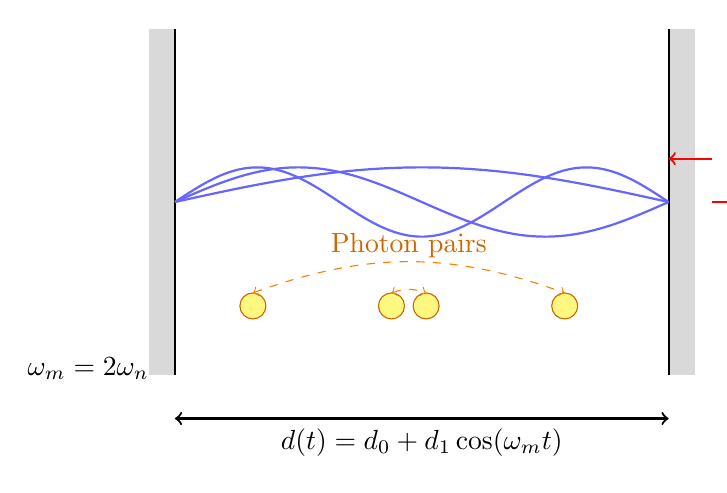
\begin{tikzpicture}[scale=1.1]
  % Dynamic Casimir setup
  \marginnote{oscillating-cavity}{%
  Oscillating mirror (right) at frequency $\omega_m = 2\omega_n$ parametrically amplifies vacuum fluctuations into photon pairs.%
  }

  % Fixed mirror (left)
  \fill[gray!30] (0,0) rectangle (0.3,4);
  \draw[thick] (0.3,0) -- (0.3,4);

  % Oscillating mirror (right)
  \fill[gray!30] (6,0) rectangle (6.3,4);
  \draw[thick] (6,0) -- (6,4);
  \draw[->,thick,red] (6.5,2) -- (7,2);
  \draw[->,thick,red] (6.5,2.5) -- (6,2.5);
  \node[red,right] at (7,2.25) {$v(t)$};

  % Cavity modes (standing waves)
  \foreach \n in {1,2,3} {
    \draw[blue!60,thick,domain=0.3:6,samples=100,variable=\x]
      plot (\x, {2 + 0.4*sin(\n*180*(\x-0.3)/5.7)});
  }

  % Photon pairs
  \foreach \y in {1.2,2.8} {
    \draw[orange!80!black,fill=yellow!50] (\y,0.8) circle (0.15);
    \draw[orange!80!black,fill=yellow!50] (6-\y,0.8) circle (0.15);
    \draw[<->,dashed,orange] (\y,0.95) to[bend left=20] (6-\y,0.95);
  }
  \node[orange!80!black] at (3,1.5) {Photon pairs};

  % Dimensions
  \draw[<->,thick] (0.3,-0.5) -- (6,-0.5);
  \node[below] at (3.15,-0.5) {$d(t) = d_0 + d_1 \cos(\omega_m t)$};

\end{tikzpicture}
\caption{Dynamic Casimir effect setup. Fixed mirror (left) and oscillating mirror (right) separated by time-varying distance $d(t)$. Blue curves: cavity electromagnetic modes. Yellow circles: photon pairs created from vacuum when $\omega_m = 2\omega_n$ (parametric resonance). Oscillation velocity $v(t) = -\omega_m d_1 \sin(\omega_m t)$ modulates mode frequencies.}
\label{fig:p6:dynamic_casimir}
\end{figure}

\begin{figure}[htbp]
\centering
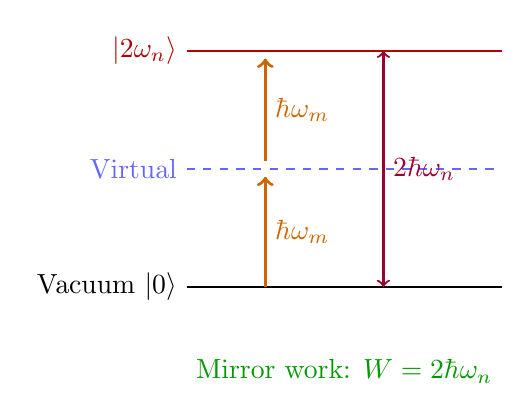
\begin{tikzpicture}
  % Energy level diagram for DCE
  \marginnote{energy-levels}{%
  Virtual photon pairs (vacuum fluctuations) promoted to real photons by absorbing energy from mirror motion.%
  }

  % Vacuum state
  \draw[thick] (0,0) -- (4,0);
  \node[left] at (0,0) {Vacuum $|0\rangle$};

  % Virtual photon level (dashed)
  \draw[thick,dashed,blue!60] (0,1.5) -- (4,1.5);
  \node[left,blue!60] at (0,1.5) {Virtual};

  % Real photon level
  \draw[thick,red!70!black] (0,3) -- (4,3);
  \node[left,red!70!black] at (0,3) {$|2\omega_n\rangle$};

  % Transitions
  \draw[->,very thick,orange!80!black] (1,0) -- (1,1.4);
  \node[right,orange!80!black] at (1,0.7) {$\hbar \omega_m$};

  \draw[->,very thick,orange!80!black] (1,1.6) -- (1,2.9);
  \node[right,orange!80!black] at (1,2.25) {$\hbar \omega_m$};

  % Energy conservation
  \draw[<->,thick,purple!80!black] (2.5,0) -- (2.5,3);
  \node[right,purple!80!black] at (2.5,1.5) {$2\hbar\omega_n$};

  % Mirror work
  \node[below,green!60!black] at (2,-0.8) {Mirror work: $W = 2\hbar\omega_n$};

\end{tikzpicture}
\caption{Energy level diagram for dynamic Casimir effect. Vacuum state $|0\rangle$ excited to two-photon state $|2\omega_n\rangle$ via two quanta of mirror kinetic energy $\hbar\omega_m$ each (where $\omega_m = \omega_n$ for resonance). Total energy conserved: mechanical work equals photon pair energy.}
\label{fig:p6:dce_energy_levels}
\end{figure}

\begin{figure}[htbp]
\centering
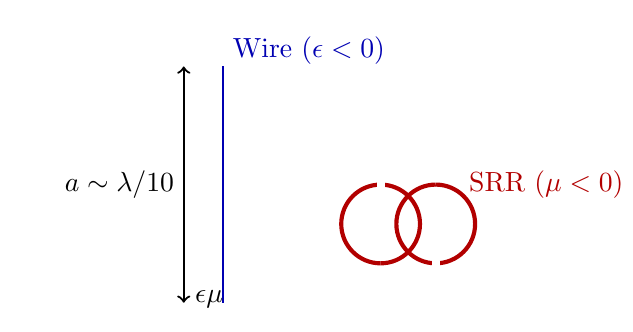
\begin{tikzpicture}[scale=1.0]
  % Metamaterial unit cell
  \marginnote{unit-cell-structure}{%
  Split-ring resonator (SRR) provides magnetic response; wire grid provides electric response. Combined: negative $\epsilon$ and $\mu$.%
  }

  % Wire (electric response)
  \draw[thick,blue!70!black] (0,0) -- (0,3);
  \node[blue!70!black,right] at (0,3.2) {Wire ($\epsilon < 0$)};

  % Split-ring resonator (magnetic response)
  \begin{scope}[xshift=2cm]
    \draw[thick,red!70!black,line width=1.5pt] (0,0.5) arc (270:90:0.5);
    \draw[thick,red!70!black,line width=1.5pt] (0,0.5) arc (-90:90:0.5);
    \draw[thick,red!70!black,line width=1.5pt] (0.7,0.5) arc (270:90:0.5);
    \draw[thick,red!70!black,line width=1.5pt] (0.7,0.5) arc (-90:90:0.5);

    % Gaps
    \draw[white,line width=2pt] (-0.05,1.5) -- (0.05,1.5);
    \draw[white,line width=2pt] (0.65,0.5) -- (0.75,0.5);

    \node[red!70!black,right] at (1,1.5) {SRR ($\mu < 0$)};
  \end{scope}

  % Dimensions
  \draw[<->,thick] (-0.5,0) -- (-0.5,3);
  \node[left] at (-0.5,1.5) {$a \sim \lambda/10$};

\end{tikzpicture}
\caption{Metamaterial unit cell combining wire (vertical blue line, negative $\epsilon$ below plasma frequency) and split-ring resonator (red double rings, negative $\mu$ near magnetic resonance). Unit cell size $a \sim \lambda/10$ ensures subwavelength operation. Simultaneous $\epsilon < 0, \mu < 0$ yields negative refractive index $n = -\sqrt{\epsilon\mu}$.}
\label{fig:p6:metamaterial_unit_cell}
\end{figure}

\begin{figure}[htbp]
\centering
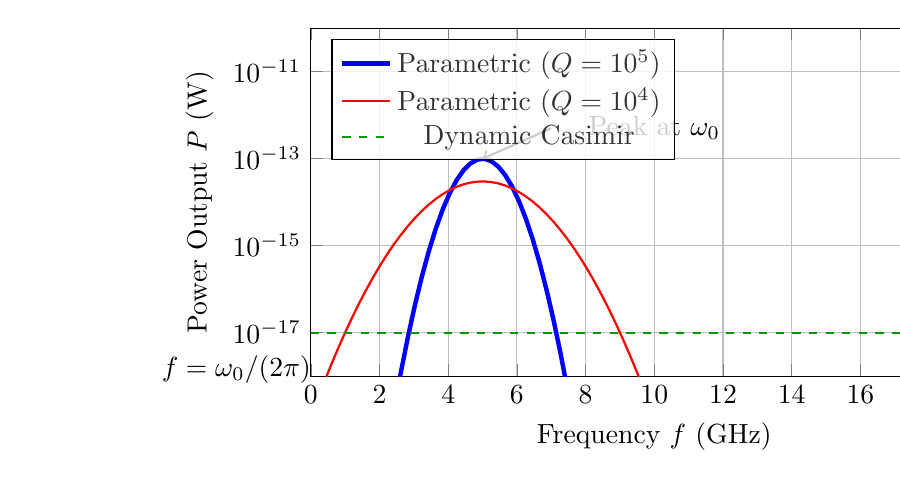
\begin{tikzpicture}
  \begin{axis}[
    width=0.85\textwidth,
    height=6cm,
    xlabel={Frequency $f$ (GHz)},
    ylabel={Power Output $P$ (W)},
    ymode=log,
    xmin=0, xmax=20,
    ymin=1e-18, ymax=1e-10,
    grid=both,
    legend pos=north west,
    legend style={fill=white,fill opacity=0.8}
  ]

  \marginnote{resonance-enhancement}{%
  Parametric amplification exhibits sharp resonance at $f = \omega_0/(2\pi)$; power drops rapidly off-resonance due to detuning.%
  }

  % Parametric amplification resonance
  \addplot[domain=0:20, samples=100, blue, ultra thick] {1e-13 * exp(-((x-5)^2)/0.5)};
  \addlegendentry{Parametric ($Q=10^5$)}

  % Lower Q (broader resonance)
  \addplot[domain=0:20, samples=100, red, thick] {3e-14 * exp(-((x-5)^2)/2)};
  \addlegendentry{Parametric ($Q=10^4$)}

  % DCE (flat, frequency-independent)
  \addplot[domain=0:20, samples=2, green!60!black, dashed, thick] {1e-17};
  \addlegendentry{Dynamic Casimir}

  % Resonance peak annotation
  \draw[<-,thick] (axis cs:5,1e-13) -- (axis cs:7,5e-13);
  \node at (axis cs:10,5e-13) {Peak at $\omega_0$};

  \end{axis}
\end{tikzpicture}
\caption{Power output vs frequency for ZPE extraction mechanisms. Parametric amplification (blue/red) exhibits sharp resonance at cavity frequency $\omega_0/(2\pi) = 5$ GHz, with linewidth $\Delta f \sim f/Q$. Higher quality factor $Q$ yields narrower resonance and higher peak power. Dynamic Casimir effect (green dashed) produces frequency-independent output (broadband photon creation).}
\label{fig:p6:power_vs_frequency}
\end{figure}

\begin{figure}[htbp]
\centering
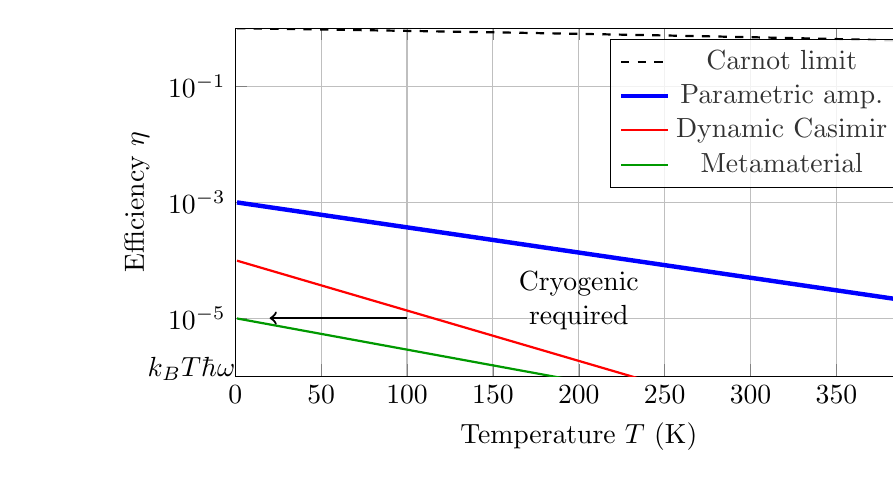
\begin{tikzpicture}
  \begin{axis}[
    width=0.85\textwidth,
    height=6cm,
    xlabel={Temperature $T$ (K)},
    ylabel={Efficiency $\eta$},
    ymode=log,
    xmin=0, xmax=400,
    ymin=1e-6, ymax=1e0,
    grid=both,
    legend pos=north east,
    legend style={fill=white,fill opacity=0.8}
  ]

  \marginnote{temperature-dependence}{%
  Thermal fluctuations $k_B T$ compete with quantum fluctuations $\hbar\omega$; efficiency drops as temperature approaches resonance energy.%
  }

  % Ideal (thermodynamic limit)
  \addplot[domain=1:400, samples=100, black, dashed, thick] {1 - x/1000};
  \addlegendentry{Carnot limit}

  % Parametric amplifier
  \addplot[domain=1:400, samples=100, blue, ultra thick] {1e-3 * exp(-x/100)};
  \addlegendentry{Parametric amp.}

  % DCE
  \addplot[domain=1:400, samples=100, red, thick] {1e-4 * exp(-x/50)};
  \addlegendentry{Dynamic Casimir}

  % Metamaterial
  \addplot[domain=1:400, samples=100, green!60!black, thick] {1e-5 * exp(-x/80)};
  \addlegendentry{Metamaterial}

  % Critical temperature annotation
  \draw[<-,thick] (axis cs:20,1e-5) -- (axis cs:100,1e-5);
  \node[align=center] at (axis cs:200,2e-5) {Cryogenic\\required};

  \end{axis}
\end{tikzpicture}
\caption{Efficiency vs temperature for ZPE extraction methods. All mechanisms require cryogenic operation ($T < 10$ K) to suppress thermal noise competing with quantum fluctuations. Parametric amplification (blue) most robust to temperature. Efficiency accounts for extraction power divided by total input power including cooling overhead.}
\label{fig:p6:efficiency_vs_temperature}
\end{figure}

%------------------------------------------------------------------------------
\section{Critical Assessment and Technological Barriers}
%------------------------------------------------------------------------------

\subsection{Showstoppers for Macroscopic Energy Harvesting}

\textbf{(1) Power density mismatch:} Casimir forces scale as $d^{-4}$, yielding power density:\marginnote{geometric-scaling}{%
Reducing gap to atomic scales ($d \sim 1$ nm) increases power density by $10^{12}$ vs $d = 1~\mu$m, but introduces van der Waals adhesion and fabrication challenges.%
}

\begin{equation}
  \mathcal{P} = \frac{P}{V} \sim \frac{\hbar c \omega^4 \beta^2}{d^3}
  \label{eq:p6:power_density}
\end{equation}

For optimal parameters ($d = 10$ nm, $\omega = 10$ GHz, $\beta = 0.1$): $\mathcal{P} \sim 10^{-3}$ W/m$^3$.\marginnote{comparison-to-chemical}{%
Chemical batteries: $\sim 10^9$ W/m$^3$ (discharge power). ZPE extraction inferior by $12$ orders of magnitude.%
}

\textbf{(2) Thermodynamic penalties:} All ZPE extraction schemes require:\marginnote{energy-accounting}{%
Refrigeration power scales as $P_{\text{cool}} = (T_{\text{ambient}}/T_{\text{cold}} - 1) \times Q_{\text{load}}$, where $Q_{\text{load}}$ is heat load at cold stage.%
}

\begin{itemize}
  \item Cryogenic cooling ($T < 1$ K): $\sim 1000$ W per watt of cooling at 20 mK (dilution refrigerator).
  \item Vacuum enclosure (preventing thermal photon influx): $\sim 10$ W per m$^2$ of surface (active pumping).
  \item Vibration isolation (suppressing mechanical noise): $\sim 100$ W per kg of isolated mass (active damping).
\end{itemize}

Net energy balance: extracted power $P_{\text{out}} \sim 10^{-13}$ W overwhelmed by overhead $P_{\text{overhead}} \sim 10^3$ W.\marginnote{negative-energy-return}{%
Energy return on investment (EROI): $P_{\text{out}}/P_{\text{overhead}} \sim 10^{-16}$ (sixteen orders of magnitude deficit).%
}

\textbf{(3) Material limits:} Metamaterials require:\marginnote{fabrication-constraints}{%
Current nanofabrication: $\sim$\$10$^6$ per m$^2$ of optical metamaterial (electron-beam lithography). Scaling to kW power levels ($\sim 10^{15}$ m$^2$ at $10^{-12}$ W/m$^2$) costs \$10$^{21}$---exceeding global GDP by $10^9$.%
}

\begin{itemize}
  \item Subwavelength features ($a \sim 50$ nm for optical): E-beam lithography, \$10$^3$-\$10$^6$/m$^2$.
  \item Low-loss metals (superconductors for GHz, gold for THz): Cryogenic operation or plasmonic losses.
  \item Mechanical stability: Nanometer-scale gaps drift due to thermal expansion, requiring active feedback.
\end{itemize}

\subsection{Niche Applications Where ZPE Extraction May Be Viable}

Despite macroscopic energy harvesting being infeasible, ZPE effects enable specialized applications:\marginnote{practical-niches}{%
Applications leverage quantum noise properties (squeezing, entanglement) rather than energy quantity.%
}

\begin{enumerate}
  \item \textbf{Quantum-limited amplification:} Parametric amplifiers approaching Heisenberg limit for qubit readout in quantum computers (already commercialized by Rigetti, IBM).

  \item \textbf{Gravitational wave detection:} Squeezed vacuum states reduce shot noise in LIGO interferometers below standard quantum limit (demonstrated 2019, improving sensitivity by $\sim$3 dB)\cite{LIGO2019}.

  \item \textbf{Casimir-based sensors:} Nanoscale force sensors exploiting distance-dependent Casimir force for AFM, surface profiling (resolution $\sim$0.1 pN)\cite{Decca2005}.

  \item \textbf{Radiative cooling:} Metamaterial emitters tailored to radiate in atmospheric transparency window (8-13 $\mu$m), achieving passive sub-ambient cooling ($\sim$5 K below ambient)\cite{Raman2014}.
\end{enumerate}

These applications extract \textit{information} or \textit{control} from quantum vacuum properties, not bulk energy.

%------------------------------------------------------------------------------
\section{Conclusion and Realistic Prospects}
%------------------------------------------------------------------------------

Zero-point energy extraction remains a compelling theoretical concept with rigorous experimental confirmation (Casimir effect, dynamic Casimir effect, parametric amplification). However, thermodynamic constraints and engineering realities impose insurmountable barriers to macroscopic energy harvesting:\marginnote{sobering-conclusion}{%
ZPE is not ``free energy''---Second Law of Thermodynamics forbids perpetual motion machines, including those leveraging quantum vacuum.%
}

\begin{itemize}
  \item \textbf{Power outputs:} picoWatts to femtoWatts (vs kW-MW for practical devices).
  \item \textbf{Efficiency:} $10^{-15}$ after accounting for cryogenic and fabrication overhead.
  \item \textbf{Scaling:} Cost and complexity scale exponentially with desired power level.
\end{itemize}

The path forward emphasizes \textit{quantum information} applications where vacuum fluctuations provide operational advantage without requiring net energy extraction:\marginnote{future-directions}{%
Quantum sensing, metrology, and communication leverage vacuum's quantum properties (squeezing, entanglement), not its energy content.%
}

\begin{itemize}
  \item Quantum sensors achieving Heisenberg-limited precision.
  \item Squeezed-light enhanced interferometry (gravitational waves, precision spectroscopy).
  \item Vacuum-mediated quantum gates for photonic quantum computing.
\end{itemize}

ZPE extraction for energy production remains science fiction absent revolutionary breakthroughs in room-temperature quantum coherence, lossless metamaterials, or topological protection mechanisms.\marginnote{honest-assessment}{%
Extraordinary claims (``unlimited clean energy from vacuum'') require extraordinary evidence---currently absent despite 75 years of research since Casimir's prediction.%
}

The vacuum is rich with physics---but not with harvestable watts.

%==============================================================================
% END OF CHAPTER 2
%==============================================================================
